\section{System Overview}


% GPS, accelerometer,magnetometer and gyroscope
 The ThunderLoc system architecture was designed to allow transmission of data from dual-microphone smartphones to the cloud platform with crowdsensing mechanism.
 %Most of smartphones have dual-microphone which provide hardware supports for our paper.
 ThunderLoc leverages stereo recording with high sampling rate of off-the-shelf mobile devices to estimate the left/right binary information.
 The perpendicular bisector of dual-microphone divides the localization space into two regions.
 If the thunder is on the right of the perpendicular bisector, then the binary code of the corresponding half-plane is set as 1, 
 and the code of the left half-plane is set as 0.


  \begin{figure}[htb]
            \setlength{\abovecaptionskip}{0pt}
            \centering
            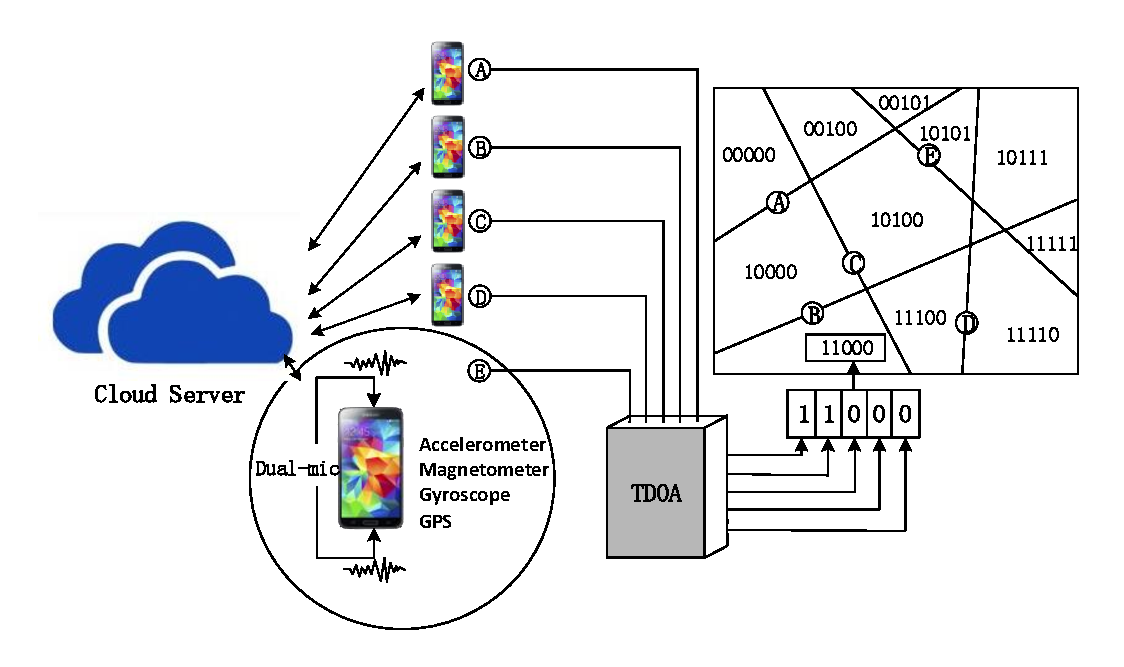
\includegraphics[scale=2,height=5.0cm]{fig/overview.pdf}
			 \vspace{1mm}
            \caption{\label{overview}System overview.}
			 \label{overview}
            \vspace{-4mm}
  \end{figure}
  
 Fig. \ref{overview} shows a layout of ThunderLoc system.  
 This research involves the use of dual-microphone smartphones as a ad-hoc sensor array based on crowdsensing in 4G cellular mobile network,
  To simplify the problem, an 2D localization space consisted of $N$ dual-microphone smartphones is considered,
 and the signals acquired by the dual-microphone of the same smartphone are synchronized.
 The perpendicular bisectors of  $N$ dual-microphones divide the localization space into some small subregions.
 
 In this paper, the thunder localization problem can be solved by using the map information and the measured binary sequence.
 Briefly, the ThunderLoc system works as shown in Fig. \ref{architecture}. 
 In the client end, the location information and direction information of the smartphone can be estimated by GPS and the motion sensors (such as accelerometer, gyroscope) integrated in the smartphone, respectively.
 When a thunder occurs, each smartphone detects TDOA of two synchronized signals recorded by dual-microphone, then achieves the binary left/right data according to the sign of TDOA.
 The APP in each smartphone uploads the 1-bit left/right binary code, the position and orientations information of the smartphone to the cloud computing platform together.
 During the data collection, participants can be even unaware of the collection task in which they are actually involved.
 Besides, ThunderLoc encourages participants to manually upload the sensing data to cloud computing platform when they hear the thunder.
 Thunder localization algorithm is run on the cloud computing platform to localize the dominant thunder.
With these random distributed smartphones, the area can be divided into subregions, according to the positions and directions of the smartphone nodes.
This naturally gives $N$-vector binary codes called the measured binary sequence in cloud computing platform,
as shown in Fig. \ref{overview}, which embedded relative position relationships among the smartphone nodes and the thunder. 
With the pre-computed subregion division, the location of the thunder can be estimated by processing the measured binary sequence.
   \vspace{-4mm}
  \begin{figure}[htb]
            \setlength{\abovecaptionskip}{0pt}
            \centering
            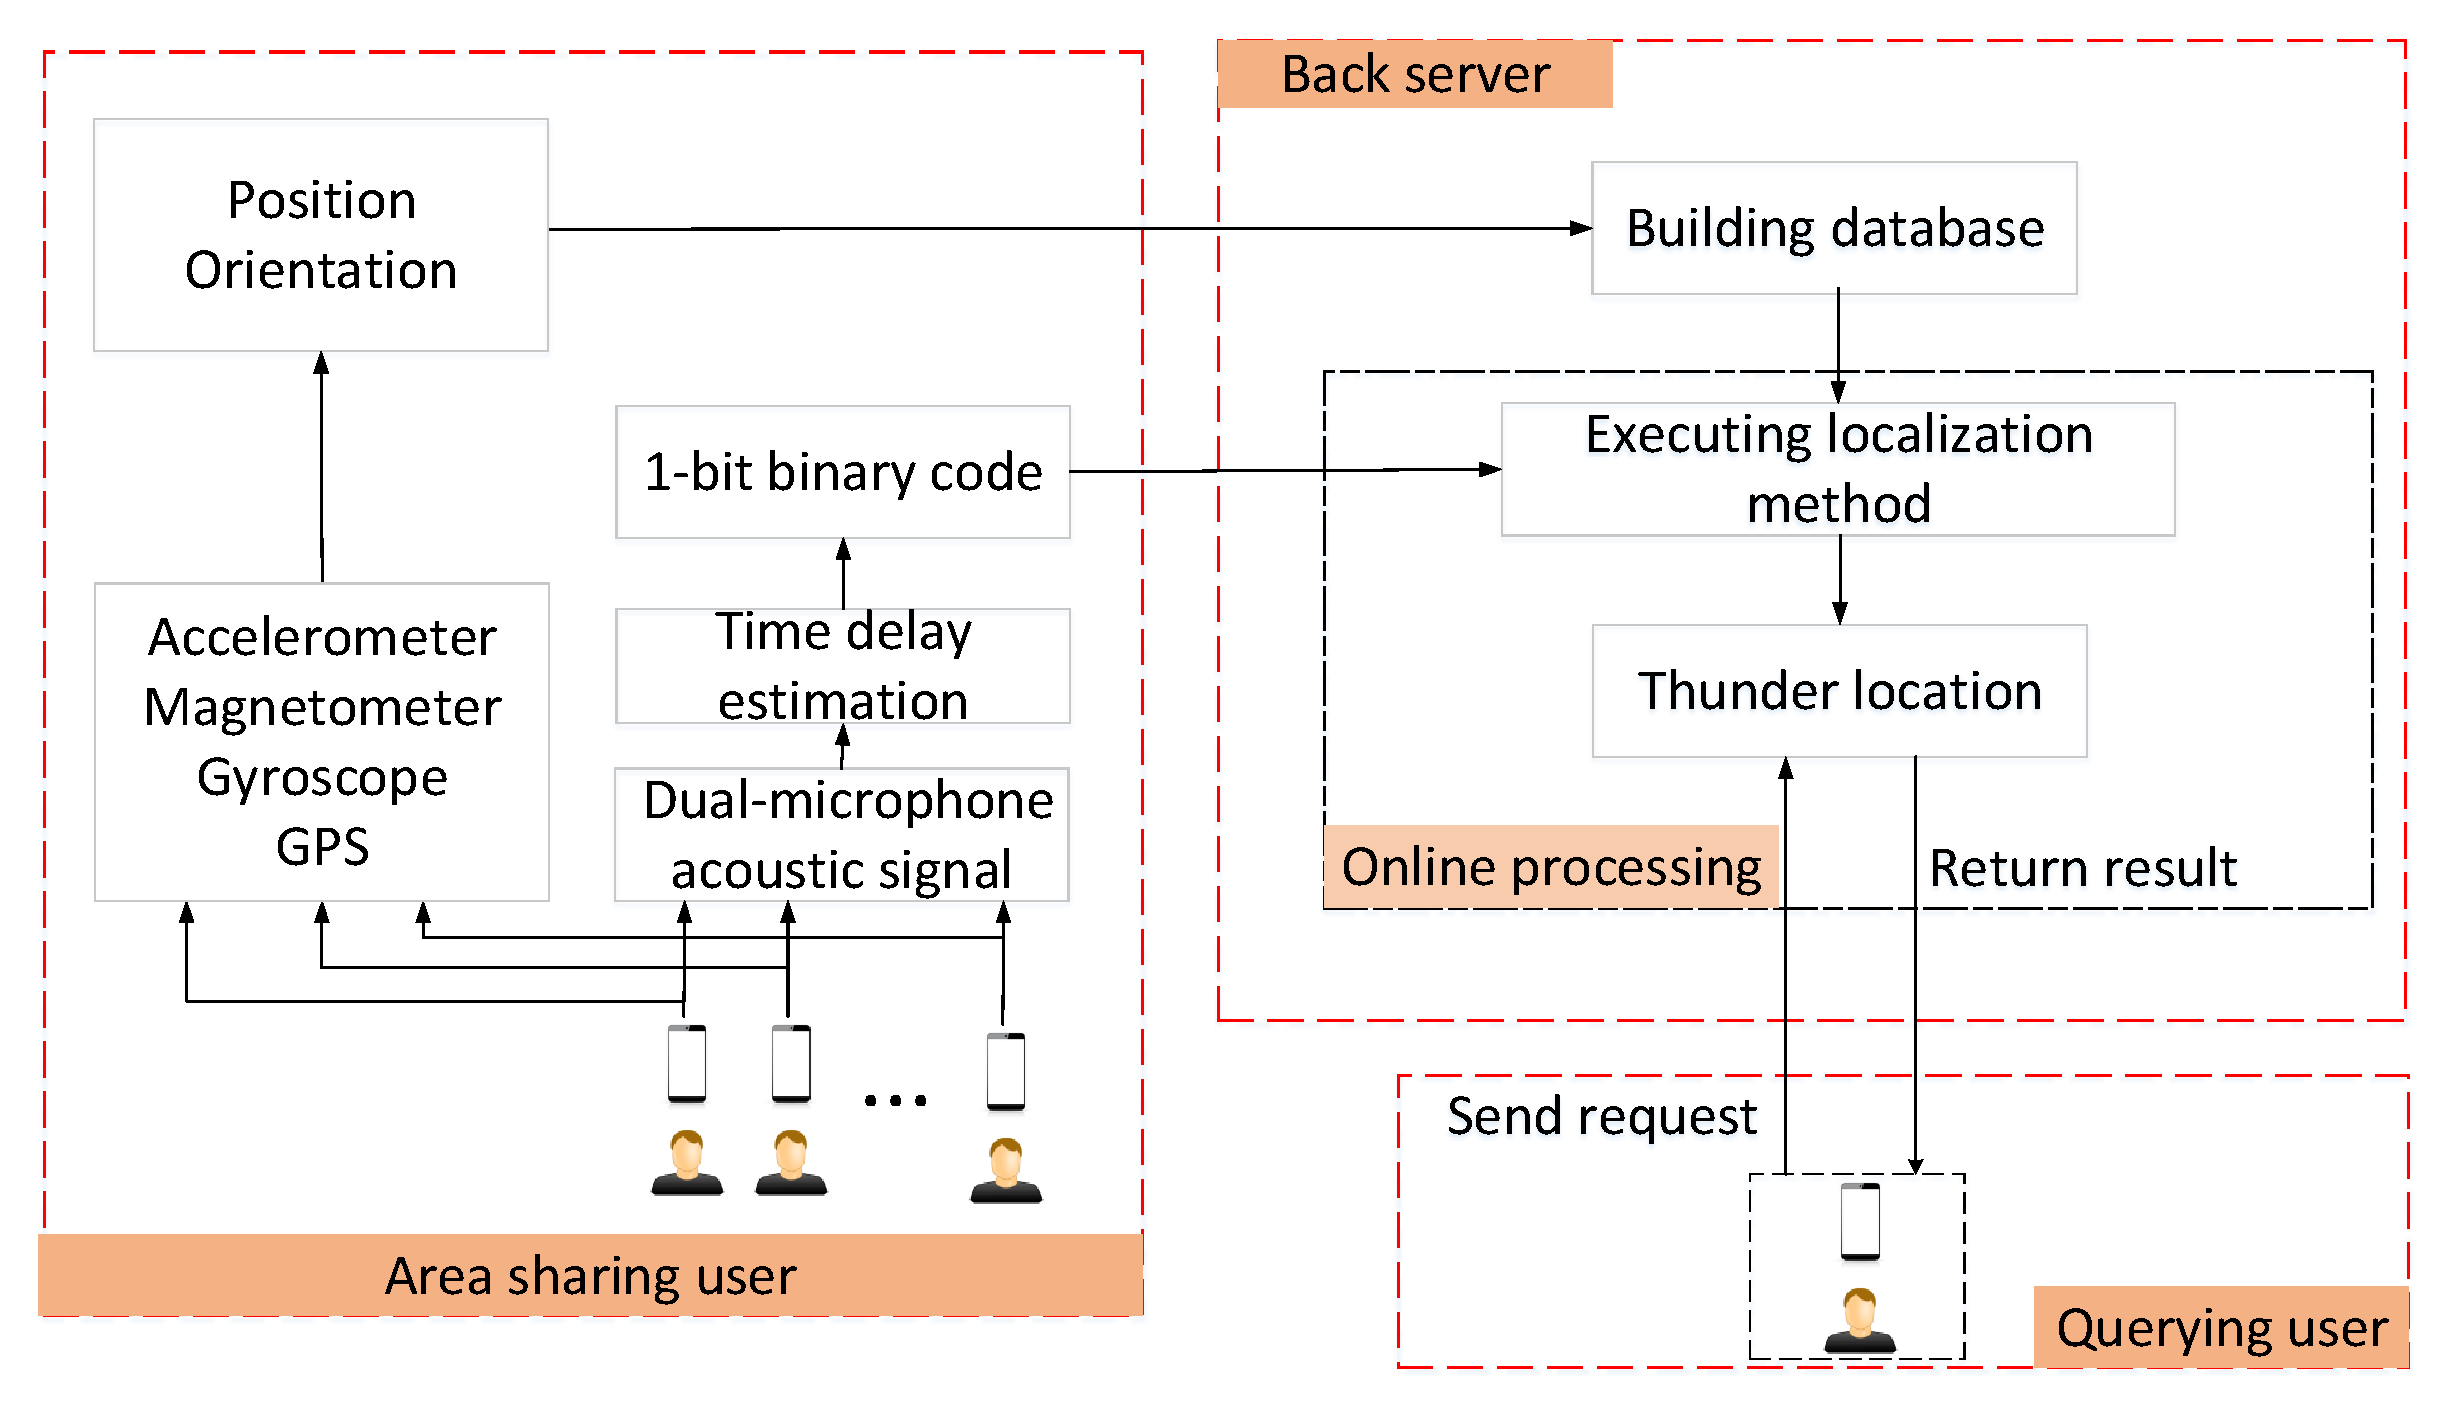
\includegraphics[scale=2,height=5.0cm]{fig/architecture.pdf}
			 \vspace{1mm}
            \caption{\label{architecture}System architecture.}
            \vspace{-4mm}
  \end{figure}
  
In the next section, we will provide the basic ThunderLoc system firstly, 
then the robust version of ThunderLoc is proposed to deal with the adverse condition in the practical application scenario.
  




